\documentclass[]{article}
\usepackage[utf8]{inputenc}
\usepackage[slovak]{babel}
\usepackage{graphicx}
\usepackage{float}
\usepackage{mathtools}
\usepackage{amsfonts}
\usepackage{tikz}
\usetikzlibrary{arrows,shapes,automata,petri,positioning}

\tikzset{
	place/.style={
		circle,
		thick,
		draw=blue!75,
		fill=blue!20,
		minimum size=6mm,
	},
	transition/.style={
		rectangle,
		thick,
		fill=black,
		minimum height=8mm,
		inner xsep=2pt
	}
}

\begin{document}
	
	
	\title{TIN - Študentská zbierka príkladov}
	\date{\today}
	
	\maketitle
	\newpage
	\tableofcontents
	\newpage
	
	\section{Chomského hierarchia}
	
	\begin{enumerate}
		\item 1. opravný termín skúšky 2017
		
		Formálne definujte pojem gramatika a pre každú triedu Chomského hierarchie uveďte typ gramatiky generujúcu jazyky tejto triedy.
		
		\item 2. opravný termín skúšky 2017
		
		Uvažujte Chomského hierarchiu jazykov rozšírenú o triedu rekurzívnych jazykov a triedu deterministických bezkontextových jazykov. Pre každú triedu tejto klasifikácie uveďte a zdôvodnite, či je v tejto triede rozhodnuteľný, alebo čiastočne rozhodnuteľný, problém náležitosti (členstva) daného reťazca do jazyka.
	\end{enumerate}

	\section{Regulárne jazyky}
	
	\begin{figure}[H]
		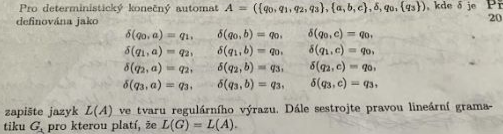
\includegraphics[width=\textwidth]{tasks/regularne/task1.png}
	\end{figure}
	
	\begin{figure}[H]
		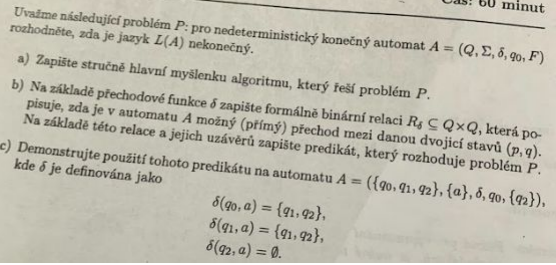
\includegraphics[width=\textwidth]{tasks/regularne/task2.png}
	\end{figure}
	
	\begin{figure}[H]
		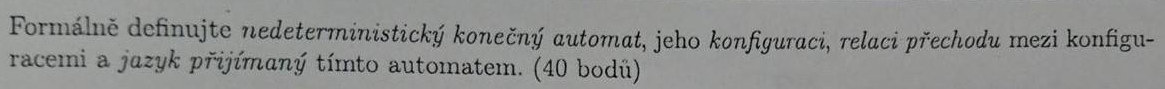
\includegraphics[width=\textwidth]{tasks/regularne/task3.png}
	\end{figure}
	
	\begin{figure}[H]
		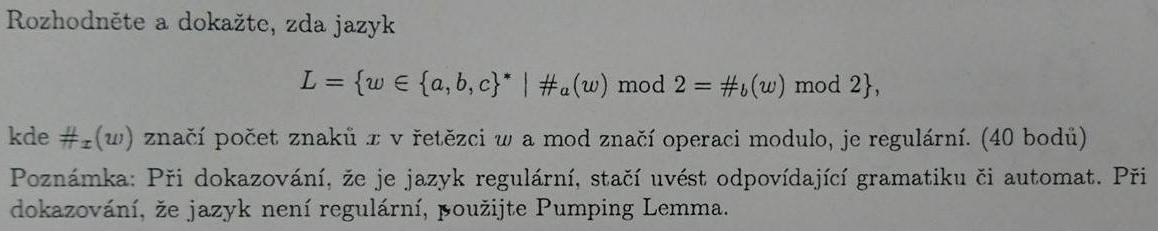
\includegraphics[width=\textwidth]{tasks/regularne/task4.png}
	\end{figure}
	
	\begin{figure}[H]
		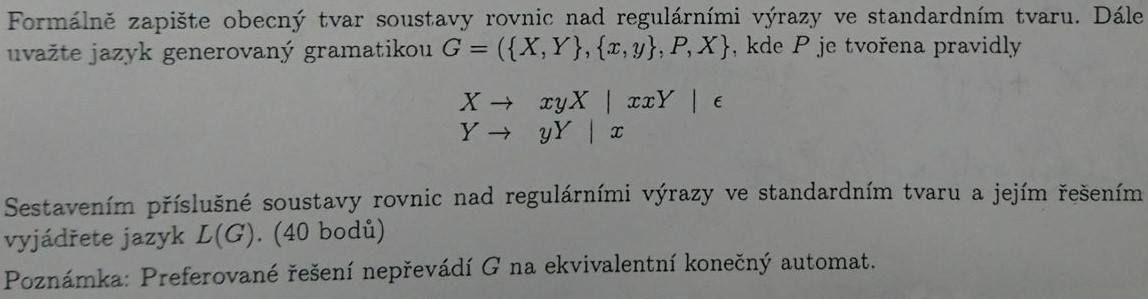
\includegraphics[width=\textwidth]{tasks/regularne/task5.png}
	\end{figure}
	
	\begin{figure}[H]
		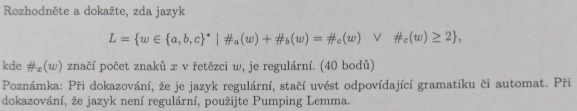
\includegraphics[width=\textwidth]{tasks/regularne/task6.png}
	\end{figure}
	
	\begin{figure}[H]
		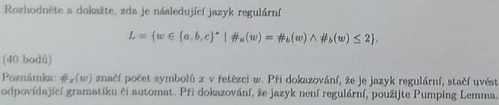
\includegraphics[width=\textwidth]{tasks/regularne/task7.png}
	\end{figure}
	
	\begin{figure}[H]
		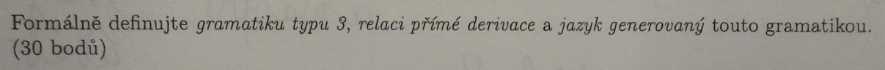
\includegraphics[width=\textwidth]{tasks/regularne/task8.png}
	\end{figure}
	
	\begin{figure}[H]
		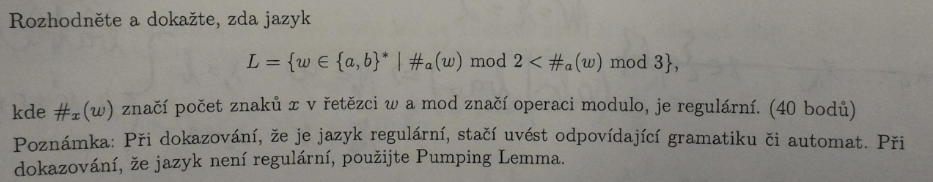
\includegraphics[width=\textwidth]{tasks/regularne/task9.png}
	\end{figure}

	\section{Bezkontextové jazyky}
	
	\begin{figure}[H]
		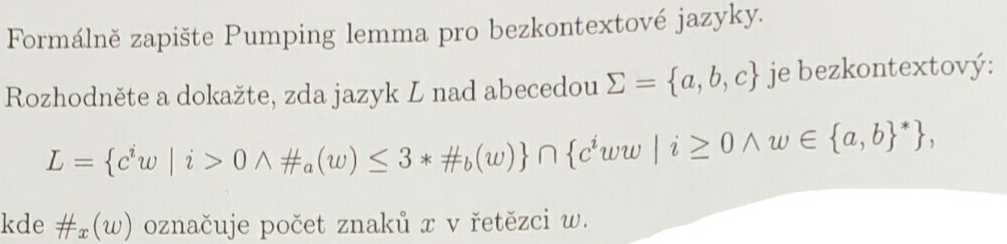
\includegraphics[width=\textwidth]{tasks/bezkontextove/task1.png}
	\end{figure}

	\begin{figure}[H]
		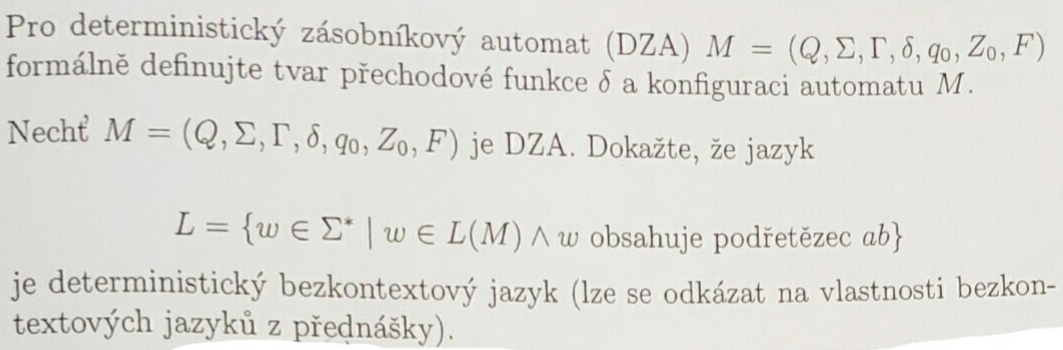
\includegraphics[width=\textwidth]{tasks/bezkontextove/task2.png}
	\end{figure}
	
	\begin{figure}[H]
		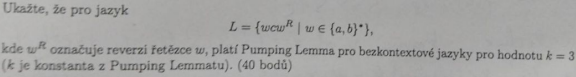
\includegraphics[width=\textwidth]{tasks/bezkontextove/task3.png}
	\end{figure}
	
	\begin{figure}[H]
		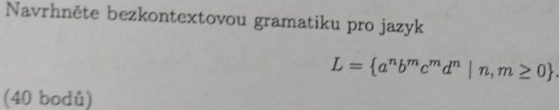
\includegraphics[width=\textwidth]{tasks/bezkontextove/task4.png}
	\end{figure}
	
	\begin{figure}[H]
		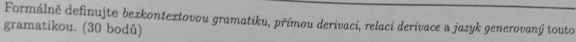
\includegraphics[width=\textwidth]{tasks/bezkontextove/task5.png}
	\end{figure}
	
	\begin{figure}[H]
		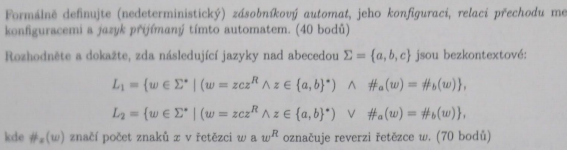
\includegraphics[width=\textwidth]{tasks/bezkontextove/task6.png}
	\end{figure}
	
	\begin{figure}[H]
		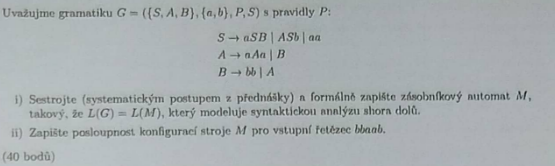
\includegraphics[width=\textwidth]{tasks/bezkontextove/task7.png}
	\end{figure}
	
	\begin{figure}[H]
		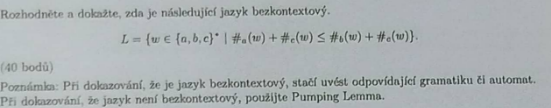
\includegraphics[width=\textwidth]{tasks/bezkontextove/task8.png}
	\end{figure}

	\begin{figure}[H]
		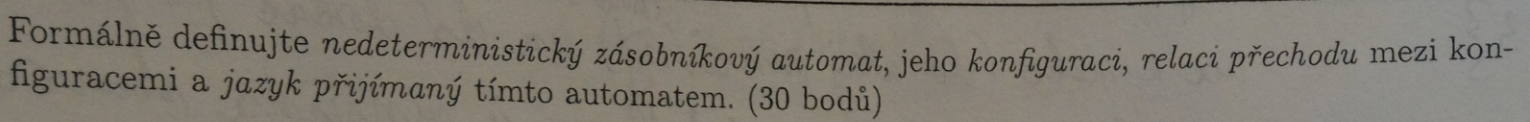
\includegraphics[width=\textwidth]{tasks/bezkontextove/task9.png}
	\end{figure}
	
	\begin{figure}[H]
		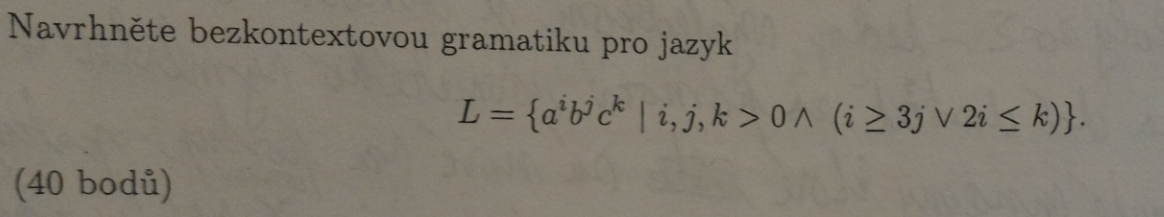
\includegraphics[width=\textwidth]{tasks/bezkontextove/task10.png}
	\end{figure}
	
	\begin{figure}[H]
		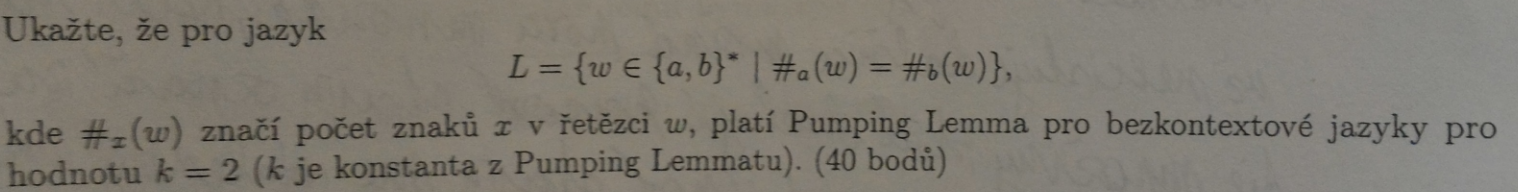
\includegraphics[width=\textwidth]{tasks/bezkontextove/task11.png}
	\end{figure}
	
	\begin{figure}[H]
		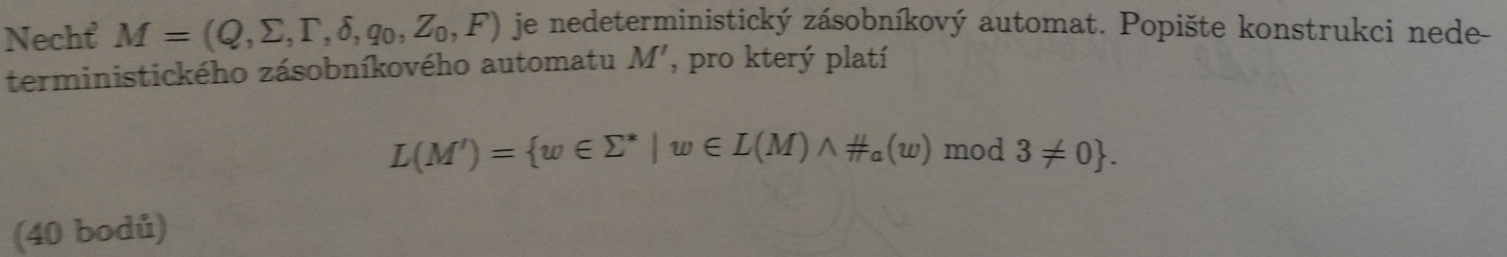
\includegraphics[width=\textwidth]{tasks/bezkontextove/task12.png}
	\end{figure}
	
	\begin{figure}[H]
		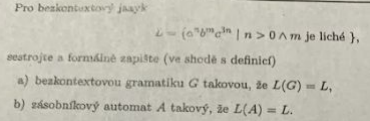
\includegraphics[width=\textwidth]{tasks/bezkontextove/task13.png}
	\end{figure}
	
	\begin{figure}[H]
		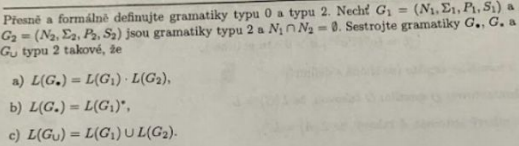
\includegraphics[width=\textwidth]{tasks/bezkontextove/task14.png}
	\end{figure}

	\section{Algoritmy}
	
	\begin{enumerate}
		\item Riadny termín skúšky 2016
		
		Definujte sústavu rovníc nad regulárnymi výrazmi v štandardnom tvare. Ďalej uvažujte obecnú lineárnu gramatiku $G$. Popíšte formálne algoritmus nájdenia regulárneho výrazu $R$ takého, že $L(G) = L(R)$, bez toho, aby bolo potrebné ku gramatike $G$ vytvárať ekvivalentný konečný automat a/alebo gramatiku $G$ transformovať. Algoritmus nájdenia regulárneho výrazu ilustrujte na príklade netriviálnej (s rekurziou, aspoň 2 nonterminály a 4 pravidla) pravej lineárnej gramatiky $G$, ktorá nie je regulárna.
		
		\item Riadny termín skúšky 2017
		
		Zapíšte algoritmus (vrátane výpočtu množiny neterminálov $N_t = \{ A \mid A \xRightarrow{}^+ \varepsilon\}$), ktorý danú bezkontextovú gramatiku transformuje na jazykovo ekvivalentnú bezkontextovú gramatiku bez epsilon pravidiel.
		
		\item 1. opravný termín skúšky 2017
		
		Formálne definujte pojem $\varepsilon$-uzáver stavu RKA (rozšíreného konečného automatu, tj. nedeterministického automate s $\varepsilon$ pravidlami) a formálne zapíšte algoritmus, ktorý v polynomiálnom čase prevedie vstupný RKA na nedeterministický konečný automat bez $\varepsilon$ prechodov (NKA). Ďalej uvažujte nasledujúci RKA $A$:
		
		\begin{center}
			\begin{tikzpicture}[scale=0.2]
			\tikzstyle{every node}+=[inner sep=0pt]
			\draw [black] (18.3,-32.8) circle (3);
			\draw (18.3,-32.8) node {$p$};
			\draw [black] (28.9,-32.8) circle (3);
			\draw (28.9,-32.8) node {$q$};
			\draw [black] (39.9,-32.8) circle (3);
			\draw (39.9,-32.8) node {$s$};
			\draw [black] (39.9,-32.8) circle (2.4);
			\draw [black] (29.7,-45.3) circle (3);
			\draw (29.7,-45.3) node {$r$};
			\draw [black] (11.2,-32.8) -- (15.3,-32.8);
			\fill [black] (15.3,-32.8) -- (14.5,-32.3) -- (14.5,-33.3);
			\draw [black] (21.3,-32.8) -- (25.9,-32.8);
			\fill [black] (25.9,-32.8) -- (25.1,-32.3) -- (25.1,-33.3);
			\draw (23.6,-32.3) node [above] {$a$};
			\draw [black] (37.437,-34.48) arc (-66.83172:-113.16828:7.72);
			\fill [black] (37.44,-34.48) -- (36.51,-34.34) -- (36.9,-35.25);
			\draw (34.4,-35.6) node [below] {$b$};
			\draw [black] (31.132,-30.831) arc (118.76404:61.23596:6.792);
			\fill [black] (31.13,-30.83) -- (32.07,-30.88) -- (31.59,-30.01);
			\draw (34.4,-29.49) node [above] {$\varepsilon$};
			\draw [black] (31.6,-42.98) -- (38,-35.12);
			\fill [black] (38,-35.12) -- (37.11,-35.43) -- (37.88,-36.06);
			\draw (35.36,-40.48) node [right] {$\varepsilon$};
			\draw [black] (20.32,-35.02) -- (27.68,-43.08);
			\fill [black] (27.68,-43.08) -- (27.51,-42.16) -- (26.77,-42.83);
			\draw (23.46,-40.51) node [left] {$\varepsilon$};
			\end{tikzpicture}
		\end{center}
		
		Pomocou zapísaného algoritmu preveďte $A$ na jazykovo ekvivalentný NKA (t.j. bez $\varepsilon$ prechodov).
		
		\item 2. opravný termín skúšky 2017, Riadny termín skúšky 2018
		
		Zapíšte algoritmus, ktorý daný nedeterministický konečný automat bez $\varepsilon$ prechodov prevedie na jazykovo ekvivalentný konečný automat. Algoritmus demonštrujte na automatu uvedenom nižšie.
		
		\begin{center}
			\begin{tikzpicture}[scale=0.2]
			\tikzstyle{every node}+=[inner sep=0pt]
			\draw [black] (18.3,-32.8) circle (3);
			\draw (18.3,-32.8) node {$1$};
			\draw [black] (28.6,-32.8) circle (3);
			\draw (28.6,-32.8) node {$2$};
			\draw [black] (28.6,-32.8) circle (2.4);
			\draw [black] (38.4,-32.8) circle (3);
			\draw (38.4,-32.8) node {$3$};
			\draw [black] (38.4,-32.8) circle (2.4);
			\draw [black] (11.2,-32.8) -- (15.3,-32.8);
			\fill [black] (15.3,-32.8) -- (14.5,-32.3) -- (14.5,-33.3);
			\draw [black] (16.977,-30.12) arc (234:-54:2.25);
			\draw (18.3,-25.55) node [above] {$a,b$};
			\fill [black] (19.62,-30.12) -- (20.5,-29.77) -- (19.69,-29.18);
			\draw [black] (21.3,-32.8) -- (25.6,-32.8);
			\fill [black] (25.6,-32.8) -- (24.8,-32.3) -- (24.8,-33.3);
			\draw (23.45,-32.3) node [above] {$a$};
			\draw [black] (31.6,-32.8) -- (35.4,-32.8);
			\fill [black] (35.4,-32.8) -- (34.6,-32.3) -- (34.6,-33.3);
			\draw (33.5,-32.3) node [above] {$b$};
			\draw [black] (37.077,-30.12) arc (234:-54:2.25);
			\draw (38.4,-25.55) node [above] {$a,b$};
			\fill [black] (39.72,-30.12) -- (40.6,-29.77) -- (39.79,-29.18);
			\end{tikzpicture}
		\end{center}
	\end{enumerate}
	
	\section{Uzáverové vlastnosti}
	
	Definujte uzavretosť triedy jazykov. Uveďte dôkaz neuzavretosti deterministických bezkontextových jazykov na operácie prienik a zjednotenie. Dokážte, že zadaná binárna relácia je uzavrená:
	
	$L_1 \circ L_2 = \{uv \mid u \in L_1 \land v \in L_2 \land \vert uv \vert \leq 5\}$.
	
	\begin{figure}[H]
		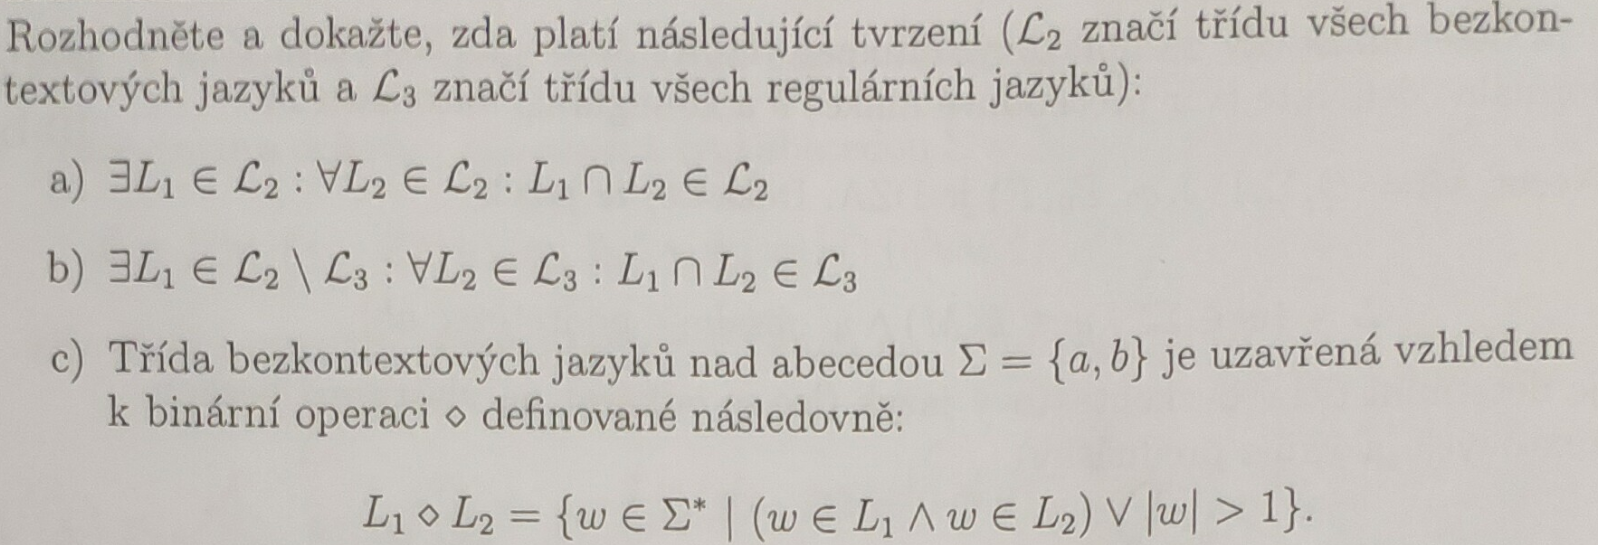
\includegraphics[width=\textwidth]{tasks/vlastnosti/task1.png}
	\end{figure}

	\begin{figure}[H]
		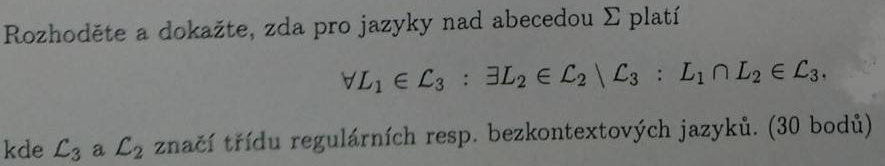
\includegraphics[width=\textwidth]{tasks/vlastnosti/task2.png}
	\end{figure}
	
	\begin{figure}[H]
		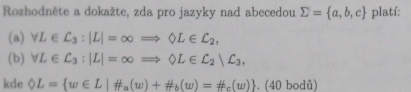
\includegraphics[width=\textwidth]{tasks/vlastnosti/task3.png}
	\end{figure}


	\begin{figure}[H]
		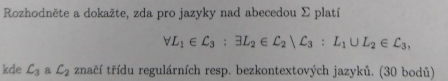
\includegraphics[width=\textwidth]{tasks/vlastnosti/task4.png}
	\end{figure}

	\begin{enumerate}
		\item Riadny termín skúšky 2018
		
		Nech $\mathcal{L}_{CK}$ značí triedu co-konečných jazykov, ktorých komplement je konečný. Rozhodnite a dokážte, či platí:
		
		$\forall L_1, L_2 \in \mathcal{L}_{CK}$ je jazyk $L_1 \cdot L_2$ regulárny
		
		\item 2. opravný termín skúšky 2017
		
		Nech $\mathcal{L}_{DBJ}$ značí triedu deterministických bezkontextových jazykov a $\mathcal{L}_{3}$ triedu regulárnych jazykov. Rozhodnite a dokážte, či platí:
		
		$\exists L_1 \in \mathcal{L}_{DBJ}: \exists L_2 \in \mathcal{L}_{3}: L_1 \cap L_2 \notin \mathcal{L}_{DBJ}$
	\end{enumerate}
	\section{Turingove stroje}
	
	\begin{enumerate}
		\item 2. priebežný test 2017
		
		Definujte prechodovú funkciu NTS, reťazec prijímaný TS, jazyk prijímaný TS. TS zadaný prechodovou funkciou má na vstupe $\Delta$abca$\Delta^{w}$. Doplňte 4 pravidlá tak, aby výstup bol $\Delta$acba$\Delta^w$.
		
		\item 2. priebežný test 2018
		
		Pre deterministický Turingov stroj $M = (Q, \Sigma, \Gamma, \sigma, q_0, q_f)$ formálne definujte tvar prechodovej funkcie $\sigma$, konfiguráciu stroja $M$ a reláciu prechodu $\vdash_M$ medzi konfiguráciami.
		
		\item 2. priebežný test 2018
		
		Zostrojte a formálne zapíšte deterministický Turingov stroj $M$ o najviac 4 stavoch a 4 prechodoch tak, aby platilo $(q_0, \Delta a^i\Delta^w, 0) {\vdash^*}_M (q_f, \Delta b^i\Delta^w, n)$, kde i,n $\geq$ 0.
	\end{enumerate}

	
	\section{Diagonalizácia}
	
	\begin{enumerate}
		\item 1. opravný termín skúšky 2017
		
		Pomocou techniky diagonalizácie dokážte, že existuje jazyk, ktorý nie je rekurzívne vyčísliteľný.
		\item Riadny termín skúšky 2016
		
		Dokážte, že existuje totálna funkcia $f: \mathbb{N} \rightarrow \mathbb{N}$, ktorá nie je primitívne rekurzívna.
		
	\end{enumerate}
	
	\section{Redukcie, rekurzívne a rekurzívne vyčísliteľné jazyky}
	\begin{enumerate}
		\item Riadny termín skúšky 2017
		
		Formálne definujte pojem redukcie jazyka $L_1$ na jazyk $L_2$ a zapíšte príslušné tvrdenia (implikácie) pre určovanie rozhodnuteľnosti resp. nerozhodnuteľnosti jazykov.
		
		\item Riadny termín skúšky 2017
		
		Rozhodnete a dokážte, či sú rekurzívne vyčísliteľné jazyky uzavreného vzhľadom k operácii pozitívna iterácia +.
		
		\item Riadny termín skúšky 2017
		
		Rozhodnite a dokážte, či existuje rekurzívne vyčísliteľný jazyk $L_1$ a rekurzívny jazyk $L_2$, pre ktoré platí $L_2 \leq L_2$ (tj. $L_1$ sa redukuje na $L_2$).
		
		\item 1. opravný termín skúšky 2017
		
		Rozhodnite a dokážte, či existuje jazyk $L$, ktorý nie je rekurzívny, ale je rekurzívne vyčísliteľný, a jeho doplnok $\overline{L}$ je tiež rekurzívne vyčísliteľný.
		
		\item Riadny termín skúšky 2016
		
		Rozhodnite a dokážte, či jazyk:
		
		$L_1 = \{\langle M \rangle \mid \exists w \in \Sigma^*$ také, že $M$ zastaví na $w\}$ je rekurzívny
		$L_2 = \{\langle M \rangle \mid \exists w \in \Sigma^*$ také, že $M$ nezastaví na $w$ behom 17 krokov$\}$ je rekurzívne vyčísliteľný
	
		$\langle M \rangle$ označuje kód Turingovho stroja so vstupnou abecedou $\Sigma$
		
		\item Riadny termín skúšky 2017
		
		Pre abecedu $\Sigma = \{a, b\}$ rozhodnite a dokážte, či:
		
		$L_1 = \{\langle M \rangle \mid M$ je Turingov stroj taký, že $\vert L(M) \cap \{a,b\} \vert = 1\}$ je rekurzívny
		
		$L_2 = \{\langle M \rangle \mid M$ je Turingov stroj taký, že $\vert L(M) \cap \{a,b\} \vert \geq 1\}$ je rekurzívne vyčísliteľný
		
		$L_3 = \{\langle M \rangle \mid M$ je Turingov stroj, pre ktorý platí, že existuje $w \in \{a,b\}^{42}$ také, že $M$ zastaví na $w$ do $\vert w \vert$ krokov$\}$ je rekurzívny
		
		Poznámka: $\langle M \rangle$ označuje kód Turingovho stroja $M$.
		
		\item 1. opravný termín skúšky 2017
		
		$L_1 = \{\langle M \rangle \mid M$ je Turingov stroj taký, že $L(M)$ je bezkontextový jazyk$\}$ je rekurzívne vyčísliteľný
		
		$L_2 = \{\langle M \rangle \mid M$ je Turingov stroj taký, že $\vert L(M) \vert \geq 3\}$ je rekurzívne vyčísliteľný
		
		Poznámka: $\langle M \rangle$ označuje kód Turingovho stroja $M$.
	\end{enumerate}
	
	\section{Zložitosť}
	
	\begin{enumerate}
		\item Riadny termín skúšky 2017
		
		Definujte formálne časovú zložitosť Turingových strojov a triedu jazykov $DTIME[n^5]$.
		
		\item Riadny termín skúšky 2017
		
		Rozhodnite a dokážte, či platí:
		
		$n^3 \in \mathcal{O}(10n^2 + 100)$
		
		$10n^2 + 100 \in \mathcal{O}(n^3)$
		
		\item Riadny termín skúšky 2017
		
		Rozhodnite a dokážte, či platí:
		
		$L_1, L_2 \in DTIME[n^3] \xRightarrow[]{} \{ uv \mid u \in  L_1 \land v \in L_2\} \in NTIME[n^3]$
		
		\item 1. opravný termín skúšky 2017
		
		Definujte formálne:
		
		\begin{itemize}
			\item pre funkciu $f: \mathbb{N} \rightarrow \mathbb{N}$ množinu $\mathcal{O}(f(n))$
			\item priestorovú zložitosť nedeterministických Turingových strojov
		\end{itemize}
	
		\item 1. opravný termín termín skúšky 2017
		
		Rozhodnite a dokážte, či platí:
		
		$L \in DTIME[n^4] \xRightarrow[]{} \{ u_1, u_2 \ldots u_k \mid k \geq 1, \forall 1 \leq i \leq k: u_i \in L\} \in NTIME[n^4]$
		
		\item Riadny termín skúšky 2018
		
		Formálne definujte:
		
		\begin{itemize}
			\item priestorovú zložitosť nedeterministických Turingových strojov, ktorý prijíma jazyk $L$
			\item asymptotické horné obmedzenie funkcie $f: \mathbb{N} \rightarrow \mathbb{N}$ (tj. $\mathcal{O}(f(n))$
			\item triedu jazykov $NSPACE[2^n]$
		\end{itemize}
	\end{enumerate}

	\section{NP problémy, polynomiálna redukcia}

	\begin{enumerate}
		\item Riadny termín skúšky 2017
		
		Definujte formálne, kedy je jazyk NP-úplný a dokážte, že nasledujúci jazyk je NP-úplný:
		
		$L = \{(\phi_1, \phi_2) \mid \phi_1, \phi_2$ sú výrokové formule v konjunktívnej normálnej forme, pre ktoré existujú dve rôzne valuácie premenných $v_1$ a $v_2$ také, že $\phi_1(v_1) \neq \phi_2(v_1) \land \phi_1(v_2) \neq \phi_2(v_2)\}$
		
		Poznámka: $\phi_i(v_i) \in \{true, false\}$ označuje, či je formula $\phi_i$ pravdivá pri valuácií premenných $v_i$.
		
		\item 1. opravný termín skúšky 2017
		
		Definujte formálne, kedy je jazyk NP-úplný a dokážte, že nasledujúci jazyk je NP-úplný:
		
		$L = \{(\phi, n) \mid \phi$ je výroková formula nad premennými $x_1, \ldots, x_k$ v konjunktívnej normálnej forme, $n \in \mathbb{N_0}$ a naviac platí, že existuje valuácia $v$ premenných $x_1, \ldots, x_k$, ktorá splňuje $\phi$, a pre ktorú platí $E(v) \geq n\}$,
		
		kde $E(v) \in \mathbb{N}$ značí číslo, ktorého binárny zápis $n_1, \ldots, n_k$ je definovaný nasledovným spôsobom:
		
		$n_i =
		\left\{
		\begin{array}{ll}
			0  & \mbox{ak } v(x_i) = true \\
			1 & \mbox{ak } v(x_i) = false
		\end{array}
		\right.$
		
		\item Riadny termín skúšky 2018
		
		Definujte formálne, kedy je jazyk NP-úplný. Ďalej uveďte hlavnú myšlienku dôkazu, že jazyk $L$ definovaný nižšie je NP-úplný:
		
		$L = \{(\phi_1, \phi_2) \mid \phi_1, \phi_2$ sú výrokové formule v konjunktívnej normálnej forme, pre ktoré existuje valuácia premenných $\vec{v}$ taká, že $\phi_1(\vec{v}) \neq \phi_2(\vec{v})\}$
		
		Poznámka: $\phi_i(\vec{v}) \in \{true, false\}$ označuje, či je formula $\phi_i$ pravdivá pri valuácií premenných $\vec{v}$.
	\end{enumerate}

	\section{Vyčíslitelné funkcie}
	
	\begin{enumerate}
		\item 1. opravný termín skúšky 2017
		
		Pomocou počiatočných funkcií a operátorov kombinácie, kompozície a primitívnej rekurzie vyjadrite funkciu:
		
		$tplus(x,y) = x + 3y$
		
		Nepoužívajte žiadne ďalšie funkcie zavedené na prednáškach mimo počiatočných funkcií. Nepoužívajte zjednodušenú syntax zápisu funkcií \-- dodržujte presne definičný tvar operátorov kombinácie, kompozície a primitívne rekurzie.
	\end{enumerate}

	\section{Petriho siete}
	
	\begin{enumerate}
		\item Riadny termín skúšky 2017
		
		Definujte formálne P/T Petriho siete. V zhode s touto definíciou popíšte sieť na obrázku (všetky miesta majú neobmedzenú kapacitu). Ďalej popíšte množinu výpočtových postupností tejto Petriho siete ako jazyk nad množinou jej prechodov.
		
		\begin{tikzpicture}[node distance=1cm,>=stealth',,bend angle=45,auto]
		\node [place,tokens=1,label=below:$P_1$] (p1) {};
		\node [transition,label=above:$T_1$] (t1) [above= of p1] {}
		edge[pre]   (p1);
		\node [transition,label=below:$T_2$] (t2) [right= of p1] {}
		edge[pre]   (p1);
		\node [transition] (t2x) [above= of p1] {}
		edge[post]   (p1);
		\node [place,label=below:$P_3$] (p3) [right= of t2] {};
		\node [transition] (t2) [right= of p1] {}
		edge[post]   (p3);
		\node [place,label=above:$P_2$] (p2) [right= of t1] {};
		\node [transition] (t1) [above= of p1] {}
		edge[post]   (p2);
		\node [transition,label=above:$T_3$] (t3) [above= of p3] {}
		edge[pre]   (p2);
		\node [transition] (t3) [above= of p3] {}
		edge[pre]   (p3);
		\node [transition] (t3x) [above= of p3] {}
		edge[post]   (p3);
		\end{tikzpicture}
		
		\item 1. opravný termín skúšky 2017
		
		Pre P/T Petriho sieť $N = (P,T,F,W,K,M_0)$ definujte formálne:
		
		\begin{itemize}
			\item predpis pre výpočet nasledujúceho značenia $M'$ zo značennia $M$ pri prevediteľnom prechode $t$ (tj. platí $M[t\rangle M'$)
			\item množinu $[M_0\rangle$ dosiahnuteľných značení siete $N$
			\item (zobecnenú) prechodovú funkciu $\sigma: [M_0\rangle \times T^* \rightarrow [M_0\rangle$
		\end{itemize}
	
		\item Riadny termín skúšky 2018
		
		Definujte formálne P/T Petriho siete. V zhode s touto definíciou popíšte sieť na obrázku (všetky miesta majú neobmedzenú kapacitu). Ďalej zapíšte prevediteľnú postupnosť prechodov a odpovedajúcich značení, v ktorej sa vyskytujú všetky prechody (použite zavedenú notáciu $M[t\rangle M'$).
		
		\begin{tikzpicture}[node distance=1cm,>=stealth',bend angle=45,auto]
		\node [place,tokens=1,label=below:$P_1$] (p1) {};
		\node [transition,label=below:$T_1$] (t1) [right= of p1] {}
		edge[pre]   (p1);
		\node [transition] (t1x) [right= of p1] {}
		edge[post]   (p1);
		\node [place,label=right:$P_2$] (p2) [above right= of t1]{};
		\node [transition] (t1) [right= of p1] {}
		edge[post, bend right]   (p2);
		\node [transition,label=above:$T_2$] (t2) [above left= of p2] {}
		edge[pre, bend left] node {3} (p2);
		\node [transition] (t2) [above left= of p2] {}
		edge[pre, bend left] node {3} (p2);
		\node [transition] (t2) [above left= of p2] {}
		edge[pre, bend right] (p1);
		\node [place,tokens=3,label=above:$P_3$] (p3) [left= of t2]{};
		\node [transition] (t2x) [right= of p3] {}
		edge[post]  node[swap] {3} (p3);
		\node [transition,label=left:$T_3$] (t3) [above left= of p1] {}
		edge[pre, bend left] node {6} (p3);
		\node [transition] (t3x) [above left= of p1] {}
		edge[post, bend right] (p1);
		\end{tikzpicture}
		
	\end{enumerate}

\end{document}